\chapter{Návrh riešenia}\label{chap:proposal}

Cieľom práce je detegovať reklamné plochy pri cestách z video nahrávky a odhadnúť ich významnosť. Kapitola je venovaná návrhu, podľa ktorého sme vypracovali riešenie.  

\section{Detekcia reklám}

Na detekciu reklám sme použili konvolučnú neurónovú sieť. Navrhli sme sieť YOLOv8 \cite{yolov8}, ktorá bola predstavená na začiatku tohto roka so sľubným vylepšením oproti predchádzajúcim verziám. Na trénovanie sme použili dataset Mapillary Vistas, ktorý bol uvedený v podobných prácach. Obsahuje 25000 obrázkov s desiatkami tried, vrátane triedy \textit{bilboard} a \textit{banner}.


\subsubsection{Sledovanie reklám}

Detektor vyhodnocuje video po jednej snímke a každá detekcia predstavuje samostatnú reklamu. Pre nás bolo dôležité detegovať trajektóriu reklamy, preto sme okrem detektora potrebovali algoritmus, ktorý identifikuje tú istú reklamu vo viacerých snímkach. Navrhli sme vyskúšať viacero sledovacích metód a porovnať ich medzi sebou.

\section{Príprava dát}

Aby sme vedeli odhadnúť významnosť reklamy, potrebovali sme mať databázu reklám s priradením významnosti, podľa ktorej by sme natrénovali klasifikátor. Keďže sme takú databázu nenašli, museli sme vytvoriť vlastnú. Pripravili sme experimentálne meranie, od ktorého sme očakávali dostatočnú kvalitu a kvantitu dát pre ďalší proces.

Na zber dát sme mali možnosť použiť eyetracker Tobii Glasses 3, ktorý je k dispozícií na našej katedre. Eyetracker je zariadenie, ktoré dokáže snímať kam sa človek pozerá a súčasne nahrávať video.

\begin{figure}[ht]
    \centering
    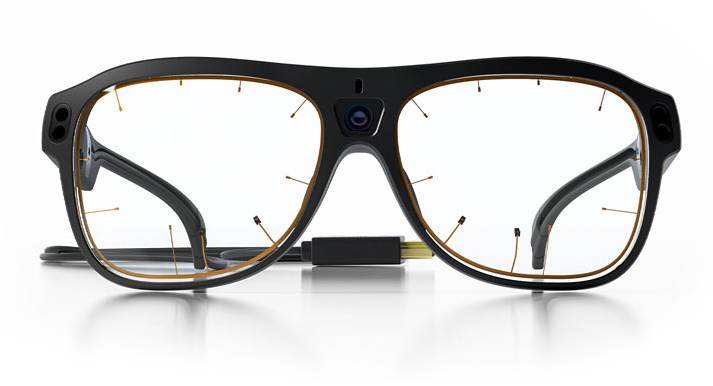
\includegraphics[width=0.5\textwidth]{images/03/glasses.jpg}
    \caption{Tobii Glasses 3 \cite{tobii}.}
    \label{img:tobii}
\end{figure}

% Potrebovali sme vytvoriť viacero záznamov jednej trasy, ktorú prejdu viacerý vodiči.

Aby bolo meranie čo najviac konzistentné, bolo dôležité zabezpečiť rovnaké podmienky pre každého účastníka merania. Na základe prečítaných prác, % ktoré robili podobný zber dát,
sme vedeli, že pohlavie neovplyvňuje meranie, preto nezáležalo na pomere pohlavia medzi účastníkmi. Naopak, to čo meranie ovplyvňuje je vek a skúsenosť so šoférovaním. Dôležitou podmienkou bola jazda v približne rovnakom počasí a hustotou premávky.

Sledovaním reklám v našom okolí, sme nakoniec zvolili okružnú jazdu, ktorá je zobrazená na obrázku \ref{img:road}. Odhadovali sme, že na zvolenej trase, ktorá trvá približne 24 minút, sa môže vyskytovať približne 150 reklamných plôch. Trasa bola zvolená kvôli rôznorodosti reklám a jej blízkosti od fakulty.

\begin{figure}[ht]
    \centering
    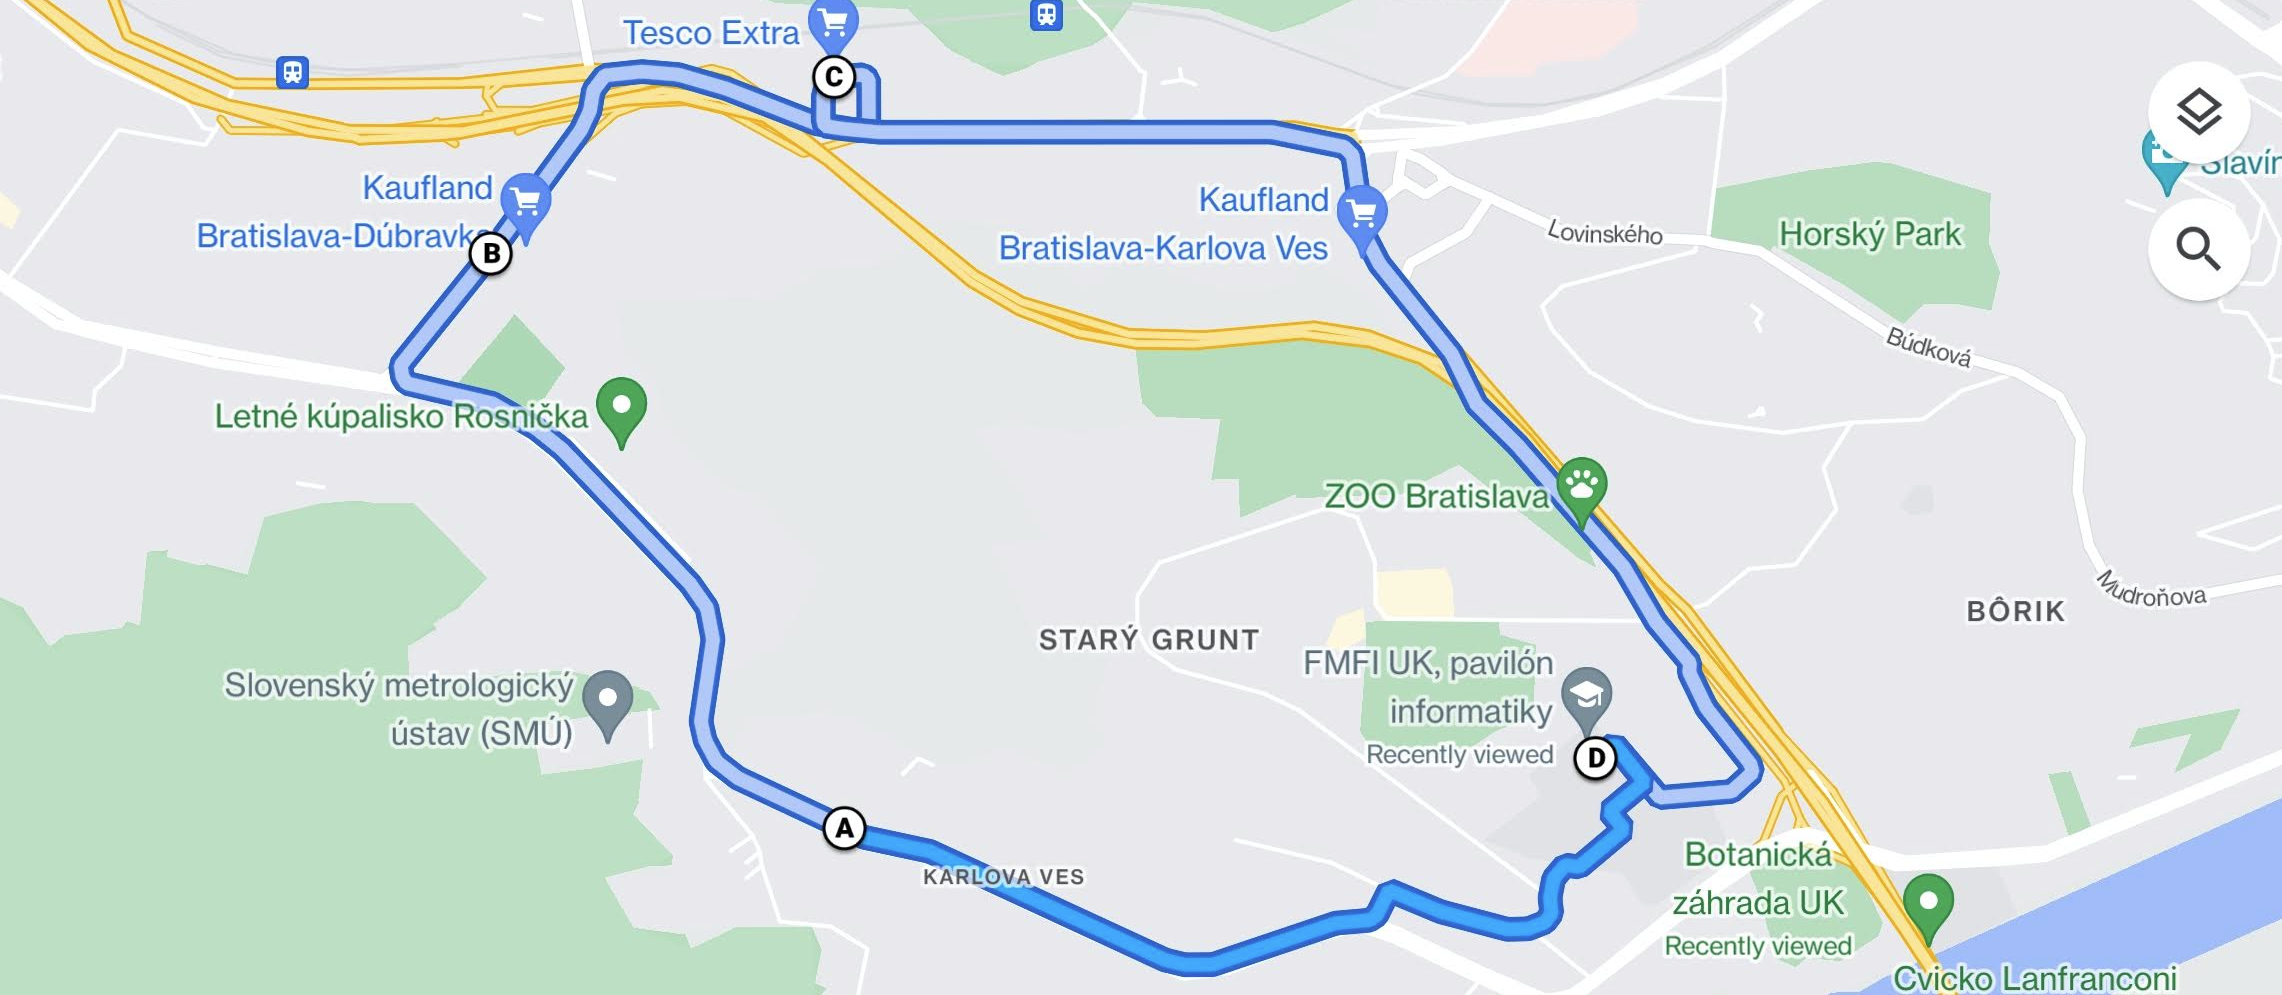
\includegraphics[width=1\textwidth]{images/03/map.png}
    \caption{Mapa trasy experimentálneho merania.}
    \label{img:road}
\end{figure}

\section{Významnosť reklám}

Spoliehali sme sa, že sledovanie dosiahne dostatočne dobrú úroveň na to, aby sme spolu s nameranými pohľadmi vodiča vedeli určiť významnosť jednotlivých reklám a tým vytvorili malú databázu reklamných plôch.

Významosť reklamy sme plánovali rozdeliť do štyroch kategórií podľa priemernej dĺžky sledovanosti:

\begin{itemize}
  \item slabá: 0ms
  \item nízka: 1 - 249ms
  \item stredná: 250 - 499ms
  \item vysoká: 500ms a viac
\end{itemize}

\section{Klasifikácia reklám}

Významnosť reklamy sme napokon potrebovali odhadnúť bez informácie o zaznamenanom pohľade vodiča. Na klasifikáciu sme použil RFC \textit{(Random forest classifier)} \cite{rfc}. Pre každú reklamu sme ako vstupné údaje do klasifikačnej metódy navrhli vypočítať nasledujúce príznaky:

\begin{itemize}
  \item počet snímok, na ktorých bola reklama viditeľná
  \item strana, na ktorej bola reklama najdlhšie
  \item priemerná vzdialenosť reklamy od stredu obrazu
  \item priemerná veľkosť reklamy
  \item priemerná hodnota mapy význačností v oblasti reklamy
\end{itemize}

% \begin{figure}[ht]
%     \centering
%     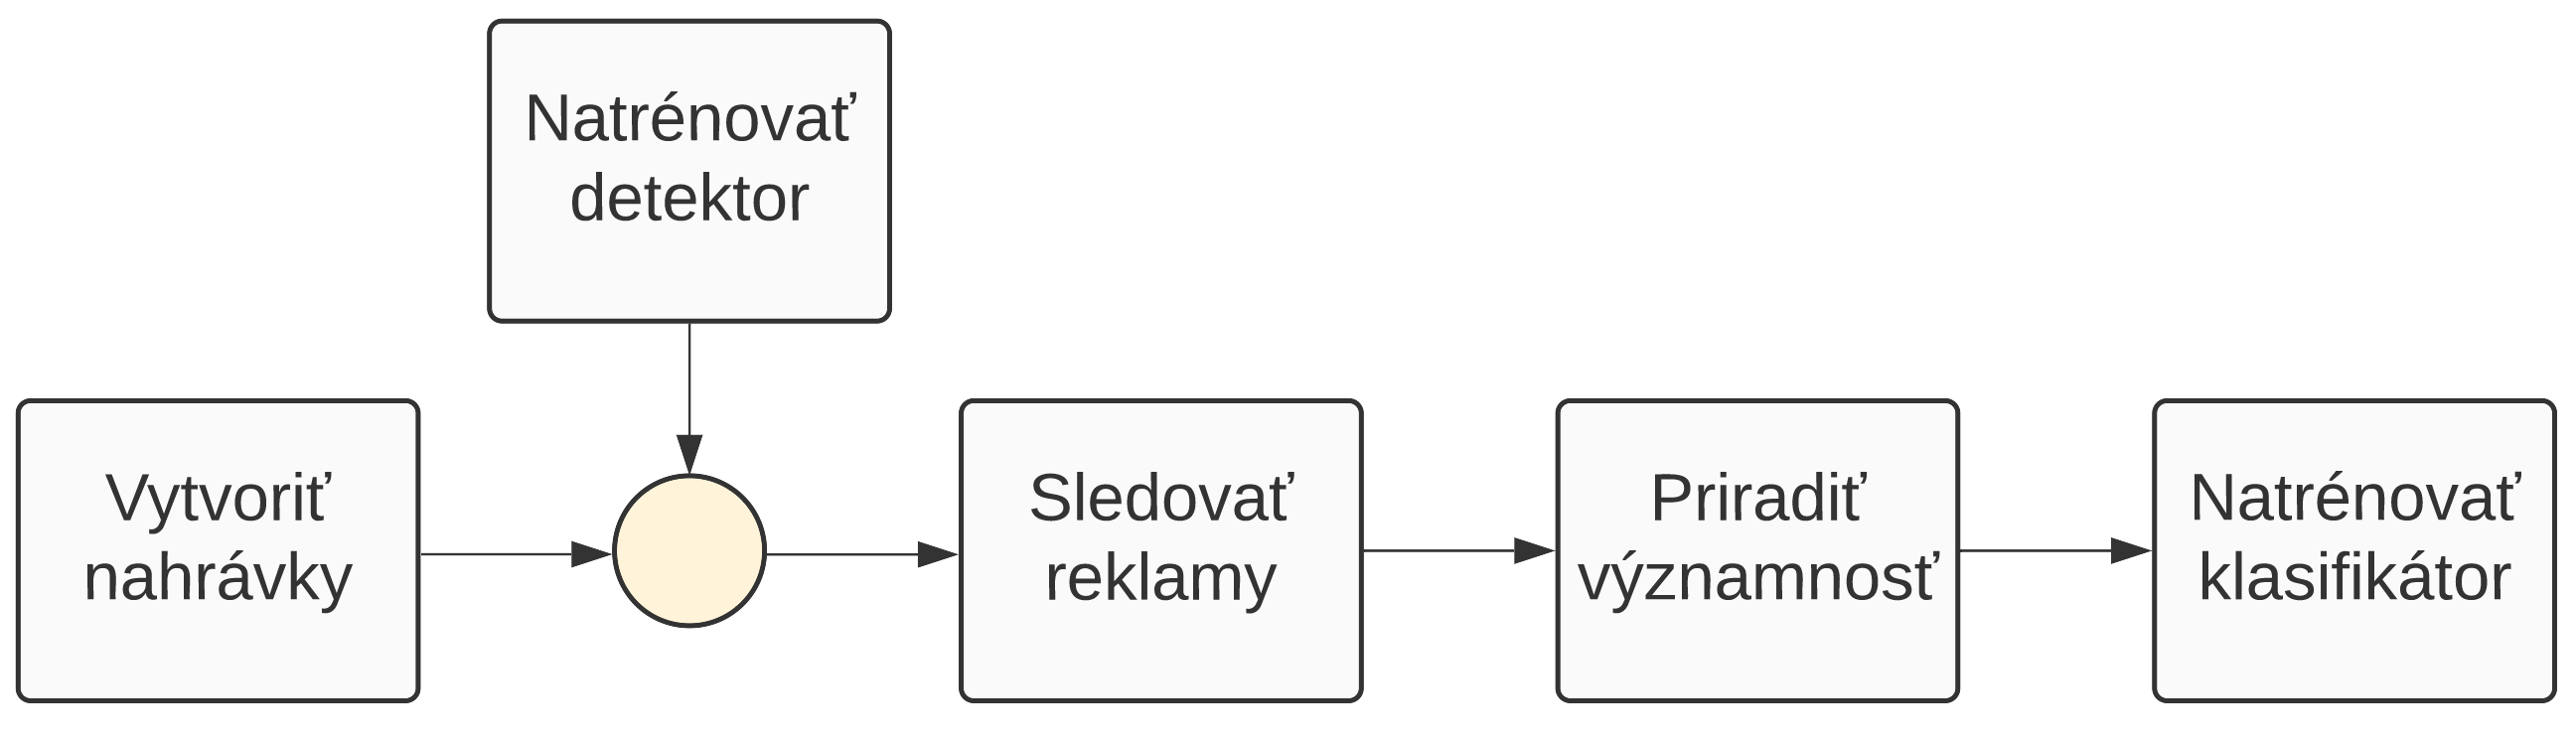
\includegraphics[width=1\textwidth]{images/02/roadmap.png}
%     \caption{Zhrnutý postup navrhnutého riešenia.}
%     \label{img:plan}
% \end{figure}